\documentclass[conference]{IEEEtran}

\usepackage[T1]{fontenc}
\usepackage[utf8]{inputenc}
\usepackage{cite}
\usepackage{url}
\usepackage{booktabs}
\usepackage{amsmath}
\usepackage{graphicx}
\usepackage{hyperref}
\usepackage{stfloats}

\newcommand{\code}[1]{\mbox{\texttt{#1}}}

\title{When Learned Monocular Priors Help: Comparing SVO and Depth Anything 3 Trajectory Estimation Across TUM and EuRoC}

\author{
\IEEEauthorblockN{Project Report Draft}
\IEEEauthorblockA{mono3d-benchmark Experimental Notes\\
June 10, 2026}
}

\begin{document}

\maketitle

\begin{abstract}
This report summarizes a practical finding from the \texttt{mono3d-benchmark} reconstruction workflow: when the input is RGB-only monocular video, using the best selected Depth Anything 3 (DA3) variant per sequence, DA3-derived camera poses achieve substantially lower Sim(3)-aligned trajectory error than the current SVO Pro Open monocular configuration on the selected TUM RGB-D sequences, while SVO remains practical and competitive when inertial measurements are available. Across the 11 EuRoC sequences already benchmarked in this repository, the mean Sim(3) trajectory error decreases from 0.898~m in monocular SVO to 0.125~m in mono+IMU SVO. A new EuRoC DA3 comparison at 5~fps and the same 30/15 chunking regime used in the TUM DA3 runs yielded a mean Sim(3) trajectory error of 2.228~m, which is substantially worse than both SVO mono and SVO mono+IMU on this dataset. In contrast, on the refreshed TUM baseline comparison, the mean Sim(3) trajectory error over the 5 directly comparable sequences is 0.429~m for SVO and 0.034~m for the best DA3 variant per sequence, a roughly 12.5$\times$ reduction in favor of DA3. Additional non-IMU SVO tuning attempts did not recover a stronger usable monocular baseline: enabling the Ceres backend was invalid without IMU in this build, loop-closure variants crashed inside SVO, and a stricter conservative monocular configuration collapsed to \code{empty\_estimate} on all six tested TUM sequences. These results support a hybrid interpretation: learned priors can be extremely effective, but their utility is model- and domain-dependent; SVO therefore remains valuable as a geometric anchor, an interpretable motion estimator, a cross-validation signal, and a tool for domain-shift analysis.
\end{abstract}

\begin{IEEEkeywords}
Monocular visual odometry, visual-inertial odometry, learned depth priors, trajectory evaluation, SVO, Depth Anything 3, TUM RGB-D, EuRoC
\end{IEEEkeywords}

\section{Introduction}
The working question behind this study was whether SVO Pro Open~\cite{forster2017svo} should remain a core trajectory source in the current monocular 3D reconstruction pipeline once Depth Anything 3 (DA3)~\cite{lin2025depthanything3} is available and functioning well. The answer matters because trajectory quality directly influences downstream dense fusion, chunk alignment, and reconstruction stability.

This question sits within a broader landscape of classical and learned SLAM and VO systems, including ORB-SLAM~\cite{mur2015orbslam}, ORB-SLAM3~\cite{campos2021orbslam3}, DROID-SLAM~\cite{teed2021droidslam}, and DPVO~\cite{teed2023dpvo}. The present report does not benchmark all of these systems directly; instead, it focuses on a practical comparison between the restored SVO path already integrated in this repository and the current DA3-based learned trajectory pipeline.

Two observations motivated the study:
\begin{enumerate}
\item SVO had already been restored and validated on EuRoC, including a working mono+IMU path.
\item DA3 was producing both useful dense reconstructions and strong trajectory estimates on TUM-prepared runs.
\end{enumerate}

The core discovery is not that SVO is broadly ineffective, but that the value of SVO depends strongly on the sensing regime. In an RGB-only monocular setting, DA3 benefits from strong learned depth priors. In grayscale or more aggressive motion regimes, however, those priors transfer less reliably. In a visual-inertial setting, SVO becomes much more competitive and practically useful.

\section{Experimental Setup}

\subsection{Classical Geometry Baseline: SVO}
The restored SVO benchmark path in this repository uses SVO Pro Open~\cite{forster2017svo} in three relevant modes:
\begin{itemize}
\item mono on EuRoC,
\item mono+IMU on EuRoC,
\item mono on TUM RGB-D, treating TUM as an RGB-only dataset for the benchmark runner.
\end{itemize}

For the TUM runs, the benchmark configuration remained monocular with the following settings:
\begin{quote}
\ttfamily\small
use\_imu: false\\
use\_ceres\_backend: false\\
runlc: false
\end{quote}
The latest TUM rerun used the official TUM RGB calibration profile written into \code{calib.yaml} for the RGB camera~\cite{tumrgbdformats}. The benchmark path does not consume TUM depth maps as input, so these runs remain monocular in the SVO sense.

\subsection{Learned Dense Baseline: DA3}
The learned baseline used DA3-LARGE through the DA3-Streaming/evaluation pipeline~\cite{lin2025depthanything3}, with matching model files and TUM evaluation scripts already integrated into this repository. For each TUM sequence, DA3 had multiple trajectory candidates produced by
\begin{itemize}
\item \texttt{fps} $\in \{2,3,5\}$,
\item \texttt{chunk:overlap} $\in \{10{:}5,20{:}10,30{:}15\}$,
\item loop-enabled DA3-Streaming trajectory estimation in the selected best-run comparison.
\end{itemize}

For the direct SVO-vs-DA3 report, the best DA3 variant per sequence was selected according to the lowest Sim(3) RMSE against TUM ground truth.

\subsection{Datasets}
Two benchmark families were used:
\begin{itemize}
\item EuRoC MAV~\cite{burri2016euroc} for assessing the value of IMU integration with SVO,
\item TUM RGB-D~\cite{sturm2012tumrgbd} for comparing RGB-only monocular SVO against DA3 on indoor RGB sequences.
\end{itemize}

The TUM sequences included:
\begin{quote}
\ttfamily\small
freiburg1\_desk\\
freiburg1\_room\\
freiburg1\_xyz\\
freiburg3\_cabinet\\
freiburg3\_large\_cabinet\\
freiburg3\_teddy
\end{quote}
The EuRoC runs used the left monocular camera stream prepared at 5~fps for the DA3 comparison, which also means that the learned baseline was evaluated in a grayscale MAV regime rather than in the indoor RGB regime where it performed best on TUM.

\subsection{Metrics}
The report relies primarily on tracking ratio, trajectory ratio, SE(3) RMSE, Sim(3) RMSE, and path-ratio-to-ground-truth. Sim(3) RMSE is emphasized because it isolates trajectory-shape fidelity after similarity alignment and therefore captures whether a monocular trajectory is structurally correct even when raw scale is imperfect. Because Sim(3) alignment corrects global scale, the reported RMSE measures trajectory-shape accuracy rather than raw metric-scale recovery.

\section{EuRoC Evidence: SVO Becomes Practical with IMU}
The first important result is that SVO should not be judged only by its monocular performance. On EuRoC, the mono+IMU configuration is markedly better than monocular SVO.

From the local EuRoC comparison summary, 11 sequences were evaluated in both modes. Mean Sim(3) RMSE dropped from 0.898~m in monocular SVO to 0.125~m in mono+IMU SVO, while the median Sim(3) RMSE dropped from 0.74~m to 0.12~m. Mean tracking ratio improved from 0.92 to 0.95, and mean trajectory ratio improved from 0.854 to 0.915. Figure~\ref{fig:euroc-sim3} visually reinforces that the IMU-backed mode consistently contracts the error distribution.

The EuRoC settings also clarify the backend story used in this project. The EuRoC mono run used:
\begin{quote}
\ttfamily\small
use\_ceres\_backend=false\\
runlc=false
\end{quote}
The EuRoC mono+IMU run used:
\begin{quote}
\ttfamily\small
use\_ceres\_backend=true\\
use\_imu=true\\
runlc=false
\end{quote}
This is consistent with the intended use of SVO as a visual-inertial system: the IMU reduces scale ambiguity, and the Ceres-backed visual-inertial path stabilizes the trajectory under conditions that are difficult for monocular feature-and-photometric tracking alone.

Relevant local artifacts include the EuRoC evaluation folder
\begin{quote}
\ttfamily\small
reports/evaluation/\\
svo\_full11\_euroc\_mono\_vs\_mono\_imu\_20260601
\end{quote}
which contains the summary table and the Sim(3), tracking-ratio, and trajectory-ratio plots.

\begin{figure}[t]
\centering

\includegraphics[width=\columnwidth]{../evaluation/svo_full11_euroc_mono_vs_mono_imu_20260601/sim3_rmse.png}
\caption{EuRoC Sim(3) RMSE comparison for SVO mono and mono+IMU.}
\label{fig:euroc-sim3}
\end{figure}

A further EuRoC check was then run with DA3-LARGE through the DA3-Streaming pipeline using the same 30/15 chunking style that worked well on TUM, but on a prepared 5~fps EuRoC frame set. The outcome was decisively negative for DA3 on this benchmark: the mean Sim(3) RMSE was 2.228~m, compared with 0.898~m for SVO mono and 0.125~m for SVO mono+IMU. DA3 beat SVO mono on only one of the 11 EuRoC sequences and did not beat SVO mono+IMU on any sequence. Figure~\ref{fig:euroc-svo-da3-sim3} is the key quantitative comparison here: it shows that the degradation is not a single outlier, but a broad pattern across the EuRoC set, with especially large errors on the harder machine-hall sequences. This matters for the paper's interpretation because it shows that learned monocular priors are not uniformly transferable across motion regimes and domains. In particular, the EuRoC test is both harder and less aligned with DA3's strongest operating regime: grayscale imagery, MAV-style motion, and more aggressive viewpoint change than the slower indoor RGB trajectories used in TUM. In other words, the TUM success of DA3 should be read as a strong in-regime result, not as evidence that classical geometry has become unnecessary.

\begin{figure*}[!t]
\centering

\includegraphics[width=0.98\textwidth]{../evaluation/euroc_svo_vs_da3_20260610T132107Z_fps5_da3_streaming/sim3_rmse.png}
\caption{EuRoC Sim(3) RMSE comparison across SVO mono, SVO mono+IMU, and DA3-LARGE through DA3-Streaming at 5~fps with 30-frame chunks, 15-frame overlap, and loop enabled. Unlike the TUM case, DA3 does not approach the visual-inertial SVO trajectory quality here and is generally worse than even monocular SVO. This is the main evidence that the DA3 prior advantage is regime-dependent rather than universal.}
\label{fig:euroc-svo-da3-sim3}
\end{figure*}

\section{TUM Evidence: DA3 Strongly Outperforms Monocular SVO}
The second major result comes from the TUM comparison between the latest monocular SVO run and the best DA3 trajectory variant per sequence.

\subsection{Sequence-Level Results}
For the refreshed baseline comparison:
\begin{table}[!t]
\caption{TUM Sequence-Level Sim(3) RMSE Comparison}
\label{tab:sequence_results}
\centering
\scriptsize
\resizebox{\columnwidth}{!}{%
\begin{tabular}{lcc}
\toprule
\textbf{Sequence} & \textbf{SVO RMSE (m)} & \textbf{DA3 RMSE (m)} \\
\midrule
\texttt{freiburg1\_desk}          & 0.4349 & \textbf{0.0203} \\
\texttt{freiburg1\_room}          & 0.9549 & \textbf{0.0832} \\
\texttt{freiburg1\_xyz}           & 0.1218 & \textbf{0.0107} \\
\texttt{freiburg3\_cabinet}        & \code{empty\_estimate} & \textbf{0.0147} \\
\texttt{freiburg3\_large\_cabinet}  & 0.2620 & \textbf{0.0303} \\
\texttt{freiburg3\_teddy}          & 0.3689 & \textbf{0.0264} \\
\bottomrule
\end{tabular}
}
\end{table}


\subsection{Aggregate Result}
On the five sequences with directly comparable non-empty SVO trajectories:
\begin{itemize}
\item mean SVO Sim(3) RMSE: 0.429~m
\item mean DA3 Sim(3) RMSE: 0.034~m
\end{itemize}

Three figures make the TUM result concrete. Figure~\ref{fig:tum-svo-da3-sim3} is the main quantitative summary across sequences. Figures~\ref{fig:tum-da3-desk-traj} and~\ref{fig:tum-svo-desk-traj} then zoom into a representative desk sequence to show what that gap looks like geometrically after Sim(3) alignment: DA3 preserves the overall loop shape more faithfully, whereas SVO follows a smoother but more drifted path.

\subsection{Best DA3 Variants Chosen}
The best DA3 runs selected by the comparison script are summarized in Table~\ref{tab:da3best}.

\begin{table}[!t]
\caption{Best DA3 TUM Trajectory Variant per Sequence}
\label{tab:da3best}
\centering
\scriptsize
\resizebox{\columnwidth}{!}{%
\begin{tabular}{llll}
\toprule
Sequence & FPS & Chunk & Overlap \\
\midrule
\texttt{freiburg1\_desk} & 2 & 30 & 15 \\
\texttt{freiburg1\_room} & 3 & 30 & 15 \\
\texttt{freiburg1\_xyz} & 2 & 30 & 15 \\
\texttt{freiburg3\_cabinet} & 2 & 30 & 15 \\
\texttt{freiburg3\_large\_cabinet} & 2 & 30 & 15 \\
\texttt{freiburg3\_teddy} & 3 & 30 & 15 \\
\bottomrule
\end{tabular}
}
\end{table}

\begin{figure*}[!t]
\centering

\includegraphics[width=0.9\textwidth]{../evaluation/tum_svo_vs_da3_baseline_20260610_091041_mono3d_tum_mono/sim3_rmse.png}
\caption{TUM Sim(3) RMSE comparison between monocular SVO and the best DA3 run per sequence. This is the main sequence-level quantitative figure supporting the TUM claim.}
\label{fig:tum-svo-da3-sim3}
\end{figure*}

\begin{figure}[!htbp]
\centering
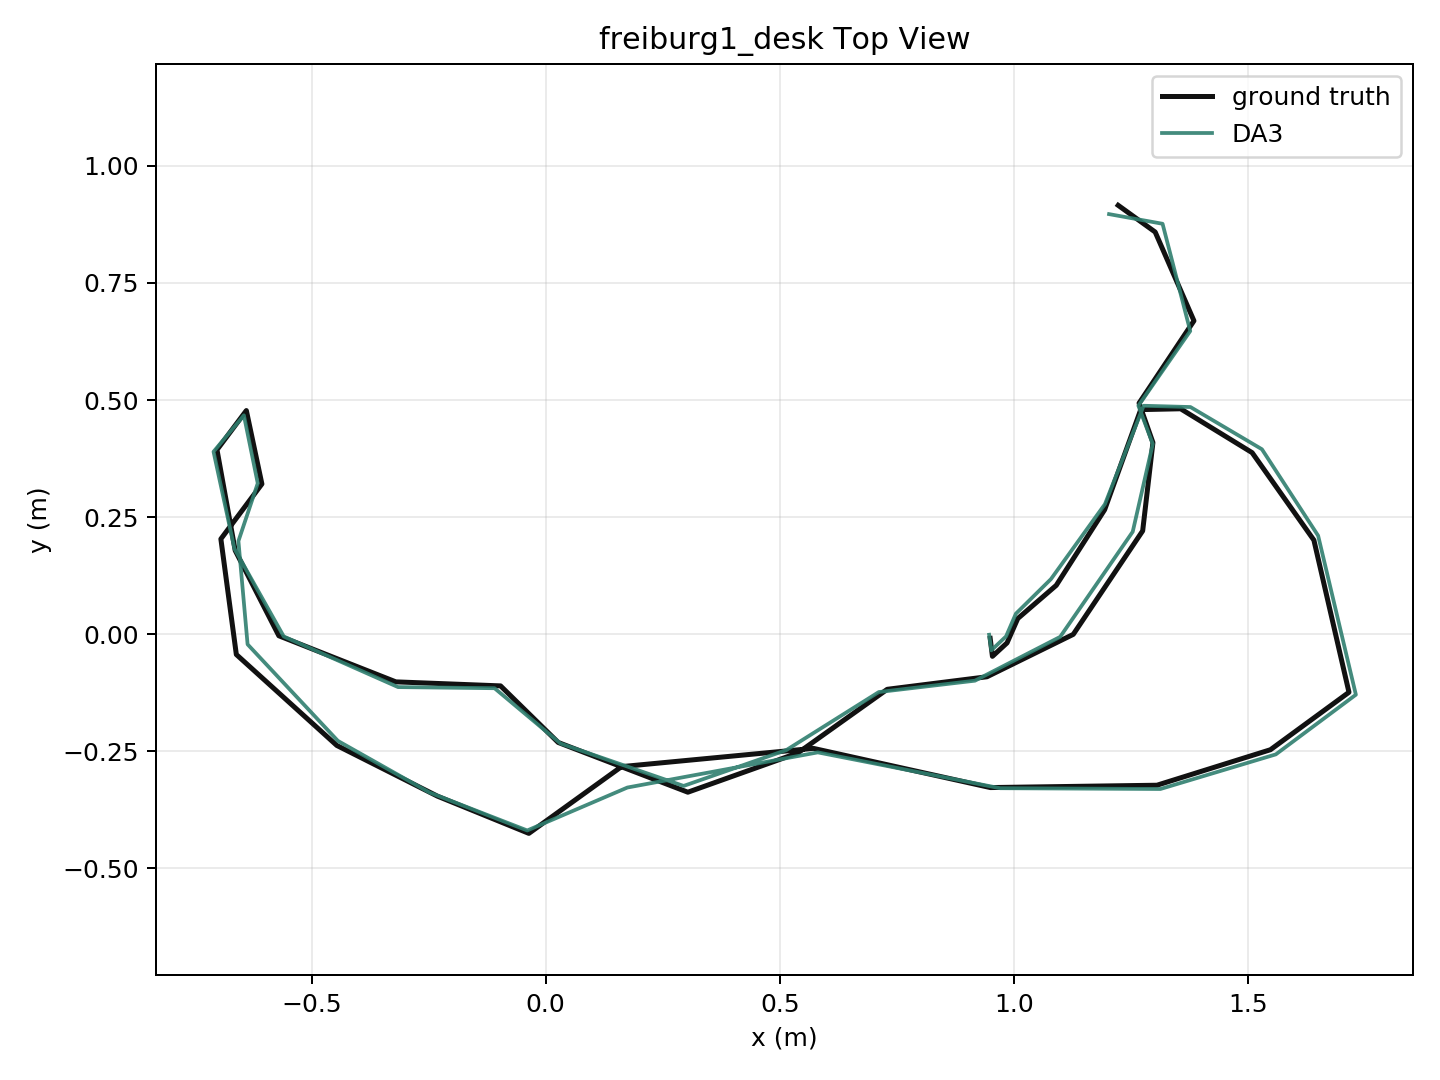
\includegraphics[width=0.95\columnwidth]{../final_comparative_report/figures/da3_freiburg1_desk_trajectory_top.png}
\caption{TUM desk sequence top-down trajectory plot for DA3 after Sim(3) alignment. The sharper corners reflect the selected keyframe path, but the global loop structure remains close to ground truth.}
\label{fig:tum-da3-desk-traj}
\end{figure}

\begin{figure}[!htbp]
\centering
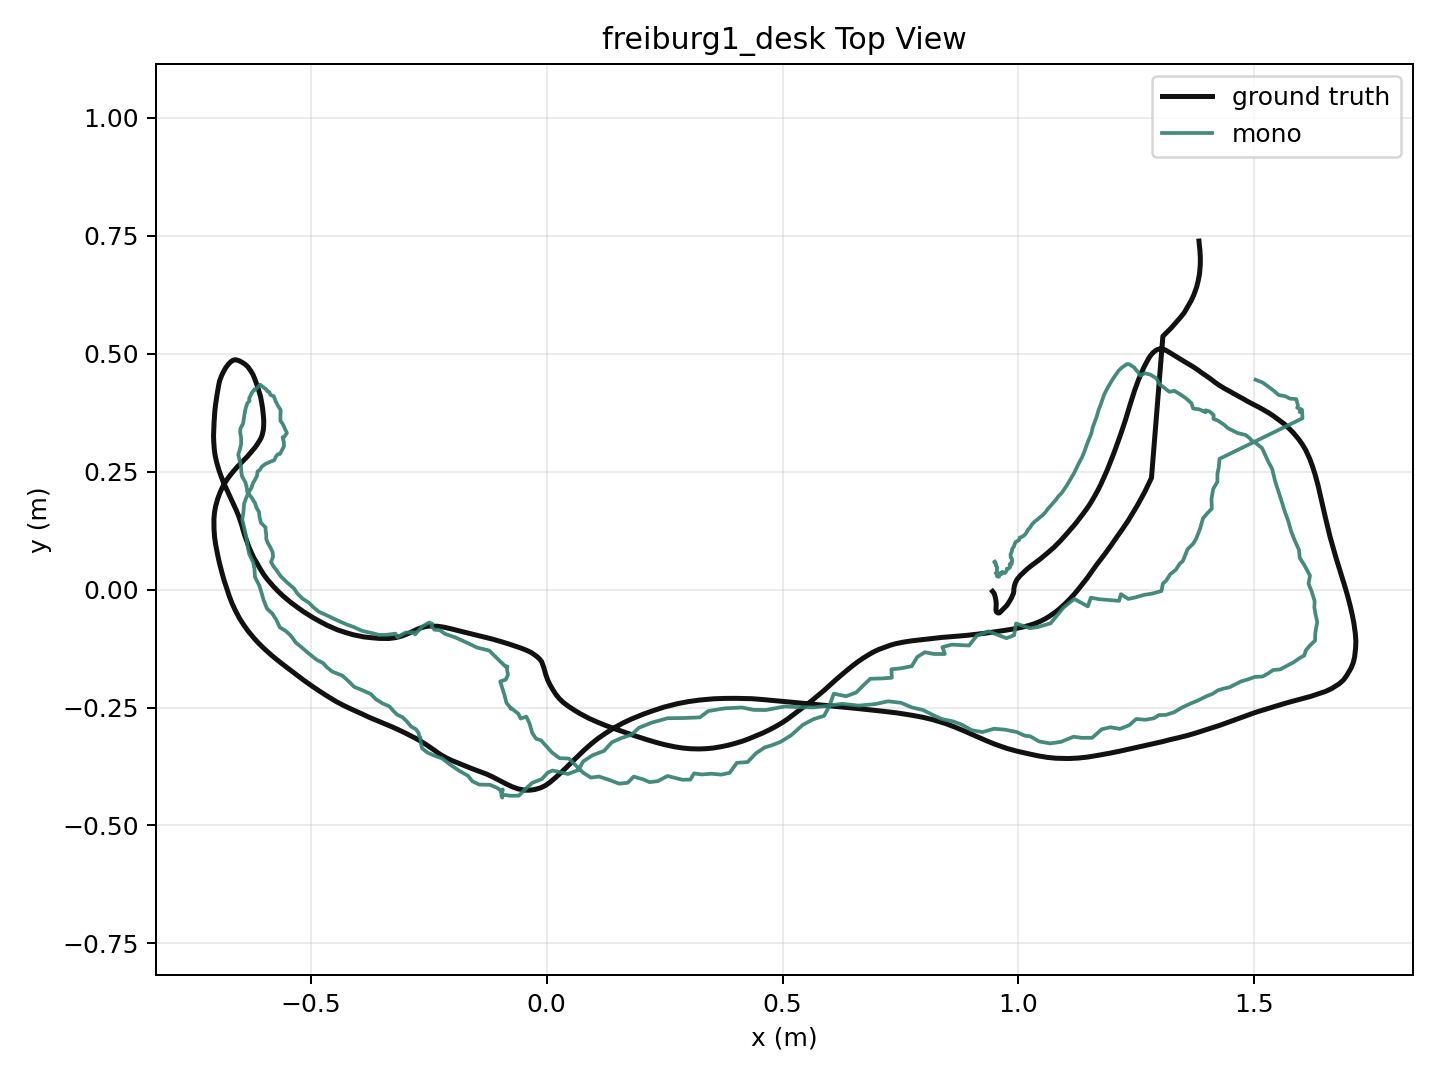
\includegraphics[width=0.95\columnwidth]{../final_comparative_report/figures/svo_freiburg1_desk_trajectory_top.png}
\caption{TUM desk sequence top-down trajectory plot for SVO after Sim(3) alignment. The SVO trajectory is visually smoother, but the accumulated drift is larger than in the DA3 estimate.}
\label{fig:tum-svo-desk-traj}
\end{figure}

This corresponds to an approximately 12.5$\times$ lower mean Sim(3) error for DA3 in this comparison. Figure~\ref{fig:tum-svo-da3-sim3} shows the gap directly at sequence level and highlights that the DA3 advantage is not tied to a single outlier sequence.

The reconstruction montage in Figure~\ref{fig:da3-reconstruction-examples} is included for a different purpose than the trajectory plots. It is not meant to replace the quantitative evaluation. Instead, it shows that the lower TUM trajectory error corresponds to qualitatively coherent 3D structure across several scene types, including the additional hall and catwalk examples from a university environment.

\begin{figure*}[!t]
\centering
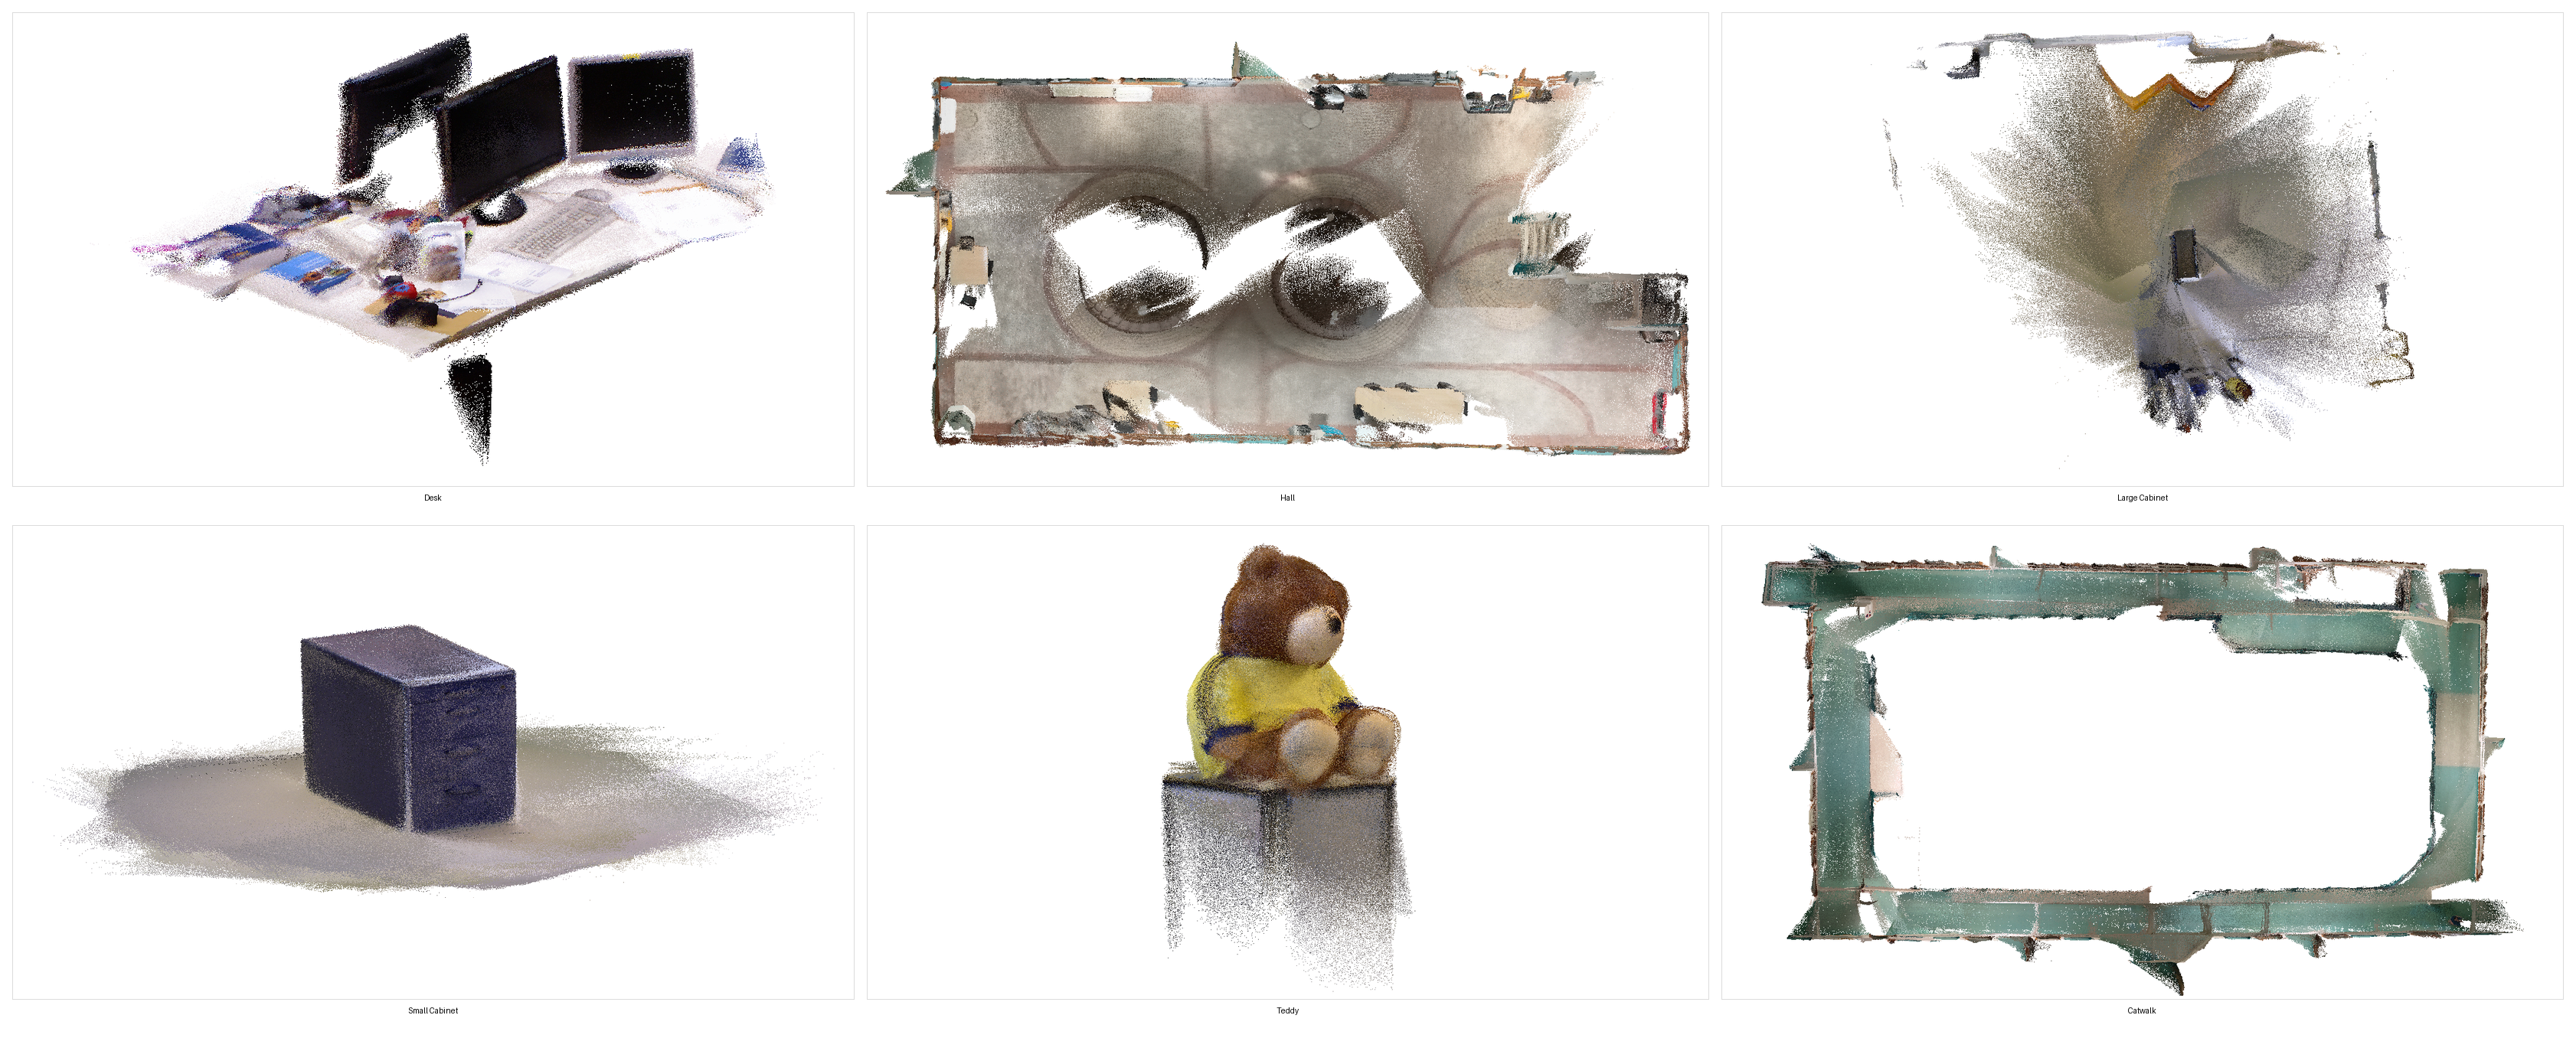
\includegraphics[width=0.98\textwidth]{figures/cloudcompare_reconstruction_grid.png}
\caption{Side-by-side qualitative DA3 reconstructions exported from CloudCompare across representative indoor and object-scale scenes. The examples show coherent recovered structure across desk, cabinet, teddy, hall, and catwalk scenes, complementing the quantitative trajectory results.}
\label{fig:da3-reconstruction-examples}
\end{figure*}

\subsection{Non-IMU SVO Tuning Attempts}
A follow-up non-IMU tuning sweep was also attempted to test whether monocular SVO could be materially improved without adding IMU information.

The practical outcome was negative. A refreshed baseline rerun improved modestly, reducing mean SVO Sim(3) RMSE from 0.4814~m to 0.4285~m, but the more aggressive non-IMU variants did not yield a stronger usable baseline. In particular, enabling the Ceres backend was not a valid monocular-only path in this SVO build because the code explicitly aborts when \code{use\_ceres\_backend=true} and \code{use\_imu=false}. Enabling loop closure in the TUM monocular path produced hard crashes inside SVO, with the failure occurring in the image-bundle processing path rather than in the surrounding benchmark scripts. A stricter conservative monocular configuration without loop closure also collapsed to \code{empty\_estimate} on all six tested TUM sequences, and its loop-enabled variant crashed in the same way as the plain loop-closure variant.

\begin{table}[!b]
\caption{Additional non-IMU SVO variants attempted on TUM}
\label{tab:svo-variants}
\centering
\small
\begin{tabular}{lp{0.45\columnwidth}}
\toprule
Variant & Outcome \\
\midrule
Baseline monocular & Usable reference run \\
Ceres without IMU & Invalid in this build \\
Loop closure & Crashed inside SVO \\
Conservative monocular & Returned \code{empty\_estimate} on all six sequences \\
Conservative + loop closure & Crashed inside SVO \\
\bottomrule
\end{tabular}
\end{table}

Therefore, the current evidence does not merely show that DA3 beats one weak monocular SVO setting. It shows that, among the practically reachable non-IMU SVO variants tested here, no stronger replacement baseline was recovered.

\section{Why DA3 Wins in the Tested RGB-Only Monocular Setting}
The practical reason for DA3's superiority on TUM is that DA3 is not solving the same inference problem as classical monocular SVO.

\subsection{Learned Depth Priors}
DA3 benefits from strong learned depth priors~\cite{lin2025depthanything3}. In this context, a depth prior is a model's built-in expectation about likely scene depth and structure learned from large-scale training data. This gives DA3 a dense geometric hypothesis even when parallax is weak, features are sparse, or texture is repetitive.

By contrast, monocular SVO must infer depth from image motion and probabilistic triangulation over time. In low-parallax or ambiguous indoor segments, this is fundamentally harder.

This also explains why the qualitative reconstruction montage in Figure~\ref{fig:da3-reconstruction-examples} matters. In a monocular pipeline, depth ambiguity makes metric structure underconstrained, and rotation-dominant motion creates a related ambiguity because pure or near-pure camera rotations provide little new baseline for triangulation. The exported DA3 reconstructions remain visually coherent across desk-scale, object-scale, and corridor-like scenes despite those conditions, which is consistent with the stronger TUM trajectory metrics. The desk, cabinet, and teddy examples connect directly to the benchmark-style indoor evaluation, while the hall and catwalk examples from a university environment are included as extra qualitative checks on reconstruction coherence outside the main TUM set. The EuRoC result shows the complementary limitation: when the input distribution shifts toward grayscale MAV imagery and harder motion, the same learned prior no longer provides a competitive trajectory estimate.

\subsection{TUM Is Unfavorable to Plain Monocular SVO in This Configuration}
The TUM benchmark path used here is RGB-only from SVO's perspective. The current benchmark integration does not consume TUM depth maps directly, and the configuration disables IMU, loop closure, and Ceres backend refinement. As a result, SVO is operating under:
\begin{itemize}
\item monocular scale ambiguity,
\item higher dependence on stable feature correspondence,
\item greater sensitivity to repeated textures and weak motion baselines.
\end{itemize}

DA3, on the other hand, often retains a coherent dense structure even under those conditions.

\subsection{Caveat: The DA3 Side Is Best-of-N}
One methodological caveat is that the DA3 comparison used the best loop-enabled trajectory variant per sequence from nine evaluated settings, whereas SVO used one shared TUM monocular configuration as the primary usable baseline. Table~\ref{tab:svo-variants} summarizes the extra non-IMU SVO variants that were also attempted and why they did not become stronger replacements. Therefore, the result should be interpreted as:

\begin{quote}
best practical DA3 trajectory found in this workflow versus a single current SVO monocular baseline.
\end{quote}

This does not weaken the central finding, but it does mean the comparison emphasizes deployable performance rather than equal hyperparameter budgets.

\section{Implications for Pipeline Design}
The results suggest that the role of SVO in the current project should be reframed.

\subsection{When DA3 Should Be Preferred}
If the immediate objective is:
\begin{itemize}
\item best monocular RGB trajectory on indoor benchmark data,
\item strong dense geometry without external IMU,
\item robust trajectory recovery under weak parallax,
\end{itemize}
then DA3 is the stronger standalone choice within the tested TUM-style RGB indoor setting. The evidence for this statement is strongest in RGB indoor scenes similar to TUM, not in every visual regime.

\subsection{When SVO Still Adds Value}
Despite this, SVO remains useful in at least four roles.

\subsubsection{Geometric Anchor}
SVO provides an explicit geometry-based trajectory estimate that can serve as an anchor or consistency signal for dense learned reconstructions, especially in environments where classical VO remains stable.

\subsubsection{Interpretability}
SVO is easier to diagnose. Failures can be linked to missing parallax, lost features, initialization instability, relocalization behavior, or scale drift. This makes it valuable for engineering and debugging even when it is not the strongest standalone trajectory source.

\subsubsection{Cross-Validation}
Agreement between SVO and DA3 increases confidence. Disagreement highlights failure cases and can trigger further inspection or fallback logic.

\subsubsection{Generalization and Domain Shift Analysis}
Learned systems often excel in-distribution but may degrade in less predictable ways under domain shift. The EuRoC result here is a concrete example: DA3 was strong on TUM RGB indoor sequences but poor on grayscale MAV imagery with harder motion, while SVO mono+IMU remained stable. Classical geometric VO, although weaker on average in some settings, provides an alternative behavior profile that can be useful for robustness studies and for understanding where learned priors help or hurt.
\section{Conclusion}
The experiments support the following conclusion.
\begin{enumerate}
\item \textbf{SVO is practical and effective when IMU is available.} The EuRoC mono+IMU results are substantially better than monocular SVO and show that SVO remains a relevant visual-inertial baseline.
\item \textbf{DA3 is clearly stronger than plain monocular SVO for trajectory estimation when the input is truly monocular RGB in the tested TUM setup.} On the refreshed baseline comparison, DA3 achieved approximately 12.5$\times$ lower mean Sim(3) RMSE than SVO over the directly comparable sequences, and it succeeded on a sequence where SVO returned an empty estimate.
\item \textbf{The explored non-IMU SVO upgrades did not overturn that result.} Ceres could not be used without IMU in this build, loop-closure variants crashed, and the stricter conservative monocular variant collapsed to empty estimates.
\item \textbf{DA3's gains are not universal across domains.} The EuRoC comparison shows that the same DA3 pipeline that performs strongly on TUM can degrade sharply under a different motion regime and dataset distribution, especially in grayscale and harder MAV-style motion, whereas SVO mono+IMU remains strong.
\item \textbf{SVO should not be discarded entirely, but its role should shift.} In the current pipeline, SVO is best justified as a geometric anchor, an interpretable motion estimator, a cross-validation signal, and a tool for generalization and domain-shift analysis.
\end{enumerate}

Accordingly, the current evidence does not support using plain monocular SVO as the primary trajectory estimator when DA3 is available and the sensing regime is monocular RGB only. It does, however, support retaining SVO as a complementary geometric component and as a stronger contender in visual-inertial scenarios, grayscale settings, and domain-shifted conditions where learned priors may transfer poorly.

\section*{Reproducibility Note}
The main local result folders referenced by this paper are the EuRoC mono-vs-mono+IMU summary, the EuRoC SVO-vs-DA3 comparison summary, the refreshed TUM monocular SVO baseline summary, and the refreshed TUM SVO-vs-DA3 comparison summary under \texttt{reports/evaluation/}. They contain the CSV summaries and evaluation plots used to support the claims in this report.

\bibliographystyle{IEEEtran}
\bibliography{ieee_svo_da3_refs_2026-06-10}

\end{document}
